%*****************************************
\chapter{Aieouad\^o's dictionary and G2P converter}\label{ch:aieouado-g2p}
%*****************************************

\footnote{This section contains is an extended version of the paper}
Aeiouad\^o is a product and an original contribution of this Master's research. It was developed by \citeauthor{Mendonca2014} \cite{Mendonca2014}, after noticing that no prior work applied machine learning algorithms to grapheme to phoneme conversion in \ac{BP}.

To the best of our knowledge, all previous efforts to solve the G2P problem in \ac{BP} used only a rule-based approach, and as such, they require complex linguistic knowledge to code rules and are difficult to evaluate. Unfortunately, it is a common practice in rule-based G2P (and a wrong one!) to develop the transcription rules based on a corpus and to evaluate them on the same corpus. This usally leads to overfitting, so that the results which are reported (some of them which approach 100\%) are hardly those which are found when such systems are applied to other data or tested in a different context. In addition to this, most of the G2P systems for \ac{BP} are proprietary or licensed under commercial terms, therefore their use is restricted.

We tried to overcome this gap by developing a hybrid G2P converter, which makes use of both rules and machine learning algorithms. The converter was evaluated with traditional machine learning metrics, such as precision, recall and F1-measure; therefore, its reported metrics are trustworthy. This converter was used to build a wide pronunciation dictionary, based on wordlist extracted from Wikipedia articles. Both the dictionary and the G2P converter are distributed under permissive licenses, respectivelly \ac{CC} and \ac{BSD}. Therefore, these resources aim at promoting the development of novel speech technologies for Brazilian Portuguese. It is interesting to notice that, despite being 6\textsuperscript{th} most spoken language in the world \cite{Ethnologue2013}, with about 200 million speakers, speech recognition and speech synthesis for Brazilian Portuguese are far from the current state of the art, specially what regard to open tools and resources \cite{Neto2011}. 

Aeiouad\^o's dictionary and G2P converter are based on the dialect of the city of S\~ao Paulo. They were designed primarily for Speech Technologies, such as \ac{ASR} an \ac{TTS}; but might also be used by linguists, speech therapists, lexicographers, students of Brazilian Portuguese as a second language, and whoever is interested in the sound structure of \ac{BP}.

The G2P converter makes use of a hybrid approach for grapheme to phoneme conversion, based on both manual transcription rules and machine learning algorithms. Hybrid approaches in grapheme to phoneme conversion have been applied successfully to other languages \cite{Damper1998, Polyakova2006, Teixeira2006, Veiga2013}. They have the benefit of taking advantage from both knowledge-based and data-driven methods. We proposed a method in which the phonetic transcription of a given word is obtained through a two-step procedure. Its primary word list derives from the Portuguese Wikipedia dump of 23\textsuperscript{rd} January 2014. We decided to use Wikipedia as the primary word list for the dictionary for many reasons: i) given its encyclopedia nature, it covers wide-ranging topics, providing words from both general knowledge and specialized jargon; ii) it contains around 168,8 million word tokens, being robust enough for the task; iii) it makes uses of crowdsourcing, lessening author's bias; iv) its articles are distributed through Creative Commons License. Wikipedia articles were transformed into plain text, tokenized and word types were extracted.

The dictionary makes use of a hybrid approach for grapheme to phoneme conversion, based on both manual transcription rules and machine learning algorithms, and aims at promoting the development of novel speech technologies for Brazilian Portuguese. Hybrid approaches in grapheme to phoneme conversion have been applied successfully to other languages \cite{Damper1998}\cite{Polyakova2006}\cite{Teixeira2006}\cite{Veiga2013}. They have the benefit of taking advantage from both knowledge-based and data-driven methods. We propose a method in which the phonetic transcription of a given word is obtained through a two-step procedure. Its primary word list derives from the Portuguese Wikipedia dump of 23\textsuperscript{rd} January 2014. We decided to use Wikipedia as the primary word list for the dictionary for many reasons: i) given its encyclopedia nature, it covers wide-ranging topics, providing words from both general knowledge and specialized jargon; ii) it contains around 168,8 million word tokens, being robust enough for the task; iii) it makes uses of crowdsourcing, lessening author's bias; iv) its articles are distributed through Creative Commons License. Wikipedia articles were transformed into plain text, tokenized and word types were extracted.

We developed a language identifier in order to detect loanwords among data. It is a known fact that when languages interact, linguistic exchanges inevitably occur. One particular type of linguistic exchange is of great concern while building a pronunciation dictionary, namely, non-assimilated loanwords \cite{Bussmann96}. Non-assimilated loanwords stand for lexical borrowings in which the borrowed word is incorporated from one language into another straightforwardly, without any translation or orthographic adaptation. These words represent a problem to grapheme-to-phoneme (G2P) conversion since they show orthographic patterns which are not predicted in advance by rules or which are too deviant to be captured by machine learning algorithms. Many algorithms have been proposed to address Language Identification (LID) from text \cite{Bergsma2012, Bilcu2006, Dolf2012, Zampieri2012}. Since our goal is to detect the language of single words, we employed n-gram character  models in the identifier, given its previous success in dealing with short sequences of characters. 

Brazilian Portuguese Phonology can be regarded as syllable and stress-driven \cite{Cristofaro2005}. In fact, many phonological processes in Brazilian Portuguese are related to or conditioned by syllable structure and stress position \cite{Girelli1990}. Vowel harmony occurs in pretonic context \cite{Bisol1989}, posttonic syllables show a limited vowel inventory \cite{Cristofaro2005}, nasalization occurs when stress syllables are followed by nasal consonants \cite{Quicoli1990}, epenthesis' processes are triggered by the occurrence of non-allowed consonants in coda position \cite{Delatorre2005} and so on and so forth. Therefore, detecting syllable boundaries and stress is of crucial importance for G2P systems, in order to achieve correct transcriptions. Several algorithms have been proposed to deal with the syllabification in Brazilian Portuguese. However most of them were not extensively evaluated nor were made publicly available \cite{Oliveira2005, Nhenhem2012, Neto2011, Rocha2013}. For this reason, we implemented our own syllabification algorithm, 
based directly on the rules of the last Portuguese Language Orthographic Agreement \cite{Acordo2009}. 

Word types recognized as belonging to Brazilian Portuguese by the language identifier were transcribed in a two-step process: i) words are submitted to a set of transcription rules, in which predictable graphemes (mostly consonants) are transcribed; ii) a machine learning classifier is used to predict the transcription of the remaining graphemes (mostly vowels). All the data were subsequently revised. Figure 1 summarizes the method.

\begin{figure}[t]
\centerline{ 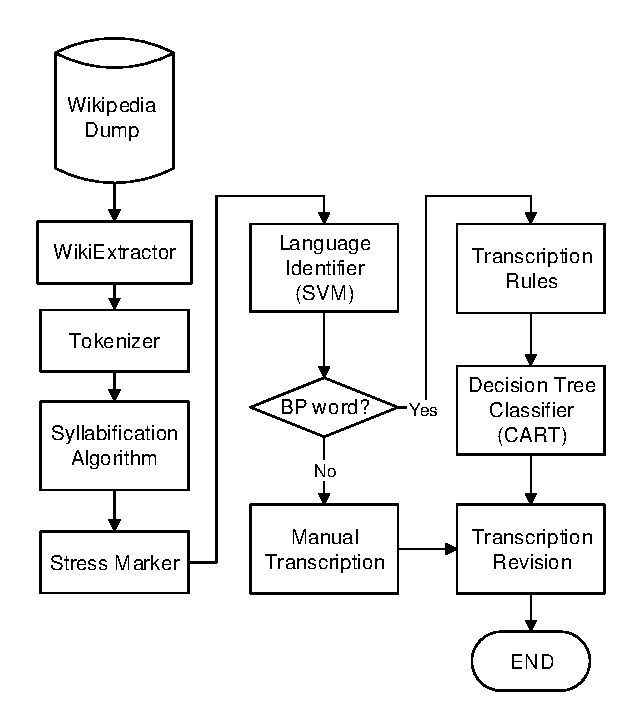
\includegraphics[width=8cm]{./gfx/aeiouado-flowchart-mod.pdf}}
\caption{{\it System architecture for building the pronunciation dictionary.}}
\label{g2p-architecture}
\end{figure}

We used the Portuguese Wikipedia's dump of 23\textsuperscript{rd} January 2014 as the primary word list for the pronunciation dictionary. In order to obtain plain text from the articles, we employed WikiExtractor \cite{Wikiextractor2013}; it strips all the  MediaWiki markups and metadata forms. Afterwards, texts were tokenized and unique words types extracted. The Portuguese Wikipedia has about 168,8 million word tokens and 9,7 million types, distributed among  820,000 articles. With the purpose of avoiding misspellings, URLs and other spurious data, only words with frequency higher than 10, which showed neither digits nor punctuation marks were selected. 

A Language Identifier module was developed in order to detect loanwords in the pronunciation dictionary. The Identifier consists of a Linear Support Vector Machine Classifier \cite{Steinwart2008} and was implemented in Python, through Scikit-learn \cite{Scikit2011}. It was trained on a corpus made of the 200,000, containing 100,000 Brazilian Portuguese words and 20,000 words of each of the following languages: English, French, German, Italian and Spanish. All of these words were collected through web crawling News' sites and were not revised. We selected these languages because they are the major donors of loanwords to Brazilian Portuguese \cite{Alves2001}. From these words we extracted features such as initial and final bi- and trigraphs;  number of accented graphs, vowel-consonant ratio; average mono-, bi- and trigraphs probability; and used them to estimate the classifier. Further details can be found in the website of the Project\footnote{http://nilc.icmc.usp.br/listener/aeiouado}. After training, we applied the classifier to the Wikipedia word list with the purpose of identifying loanwords among data. The identified loanwords were then separated from the rest of words for later revision, i.e. they were not submitted to automatic transcription.

Our syllabification algorithm follows a rule-approach and is based straightforwardly on the syllabification rules described in the Portuguese Language Orthographic Agreement \cite{Acordo2009}. Given space limitations, rules were omitted from this paper as they can be found in the website of the project, along with all the resources developed for the dictionary. As for the stress marker, once the syllable structure is known in Brazilian Portuguese, one can predict where stress falls. Stress falls:

\begin{enumerate}
 \item on the antepenultimate syllable if it has an accented vowel $<$\'a,\^a,\'e,\^e,\'i,\'o,\^o,\'u$>$;
 \item on the ultimate syllable if it contains the accented vowels $<$\'a,\'e,\'o$>$ or $<$i,u$>$; or if it ends with one of the following consonants $<$r,x,n,l,z$>$;
 \item on the penultimate syllable otherwise.
\end{enumerate}

The transcriber is based on a hybrid approach, making use of manual transcription rules and an automatic classifier, which builds Decision Trees. Initially, transcription rules are applied to the words. The rules covers not all possible graphemes to phoneme relations, but only those which are predictable by context. The output of the rules is what we called the intermediary transcription form. After obtaining it, a machine learning classifier is applied in order to predict the transcription of the remaining graphemes. Figure 2 gives an example of the transcription process.

\begin{figure}[!ht]
\centerline{ 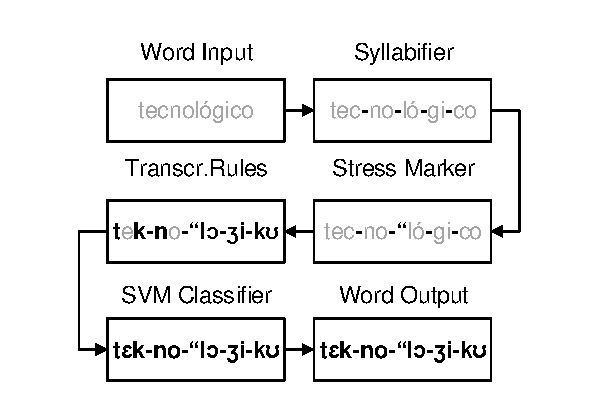
\includegraphics[width=8cm]{./gfx/aeiouado-transcript-ex.pdf}}
\caption{{\it Example of the transcription procedure -- in grey: graphemes yet to be transcribed; in black: graphemes already transcribed.}}
\label{transcExample}
\end{figure}

The rules' phase has two main goals: guarantee the correct transcription of certain predictable graphemes (mostly consonants) and also ensure the alignment between graphemes and phones for the classifier. They were set in order to avoid overlapping and order conflicts. Long sequences of graphemes, such as triphthongs, contextual diphthongs and general diphthongs are transcribed first (e.g.  $<$x-ce$> \rightarrow $\textipa{[-se]}). Then graphemes involving phones that undergo phonological processes are transcribed (e.g. $<$ti$> \rightarrow $\textipa{[tSi]}, $<$di$> \rightarrow $\textipa{[dZi]}). After that, several contextual and general monophones are transcribed (e.g. $<$\#x$> \rightarrow $\textipa{[S]}, $<$\#e-x$> \rightarrow $\textipa{[}\#\textipa{e-z]}). 

On what regards to the classifier, it was developed primarily to deal with the transcription of vowels. In Brazilian Portuguese, vowels have a very irregular behavior, specially the mid ones. Therefore the relations between the vowels' graphemes and their corresponding phonemes are hard to predict beforehand through rules. Consider, for instance, the words ``teto'' \emph{(roof)} and ``gueto'' \emph{(ghetto)}; both are nouns and share basically the same orthographic environment. However the former is pronounced with an open ``e'' \textipa{["tE.tU]} and the latter with a closed one \textipa{["ge.tU]}. The classifier employs Decision Trees, through an optimised version of the CART (Classification and Regression Trees) algorithm and was implemented in Python, by means of the Scikit-learn library \cite{Scikit2011}. 

The algorithm was trained over a corpus of 3,500 words phonetically transcribed and manually revised, with a total of 39,934 instances of phones. The feature extraction happened in the following way. After reviewing the data, we obtained the intermediary transcription form for each of these words and aligned them with the manual transcription. Then, we split the intermediary transcription form into its corresponding phones and, for each phone, we extracted the following information: 

\begin{enumerate}
 \item the phone itself; 
 \item 8 previous phones; 
 \item 8 following phones; 
 \item the distance between the phone and the tonic syllable; 
 \item word class -- parts of speech; 
 \item the manually transcribed phone. 
\end{enumerate}

We considered a window of 8 phones in order deal with vowel harmony phenomena. By establishing a window with such length, one  can assure that pretonic phones will be able to reach the transcription of the vowels in the stressed syllable. The classifier was applied to all 108,389 words categorized as BP words by the Language Identifier module, all of them were cross-checked by two linguists with experience in Phonetics and Phonology.

The Portuguese Wikipedia has about 168,8 million word tokens and 9,7 million types, distributed among 820k articles. After applying the filters to the data, i.e. words with frequency higher than 10, with no digits nor punctuation marks, we ended up with circa 238k word types, representing 151,9 million tokens. Table 1 describes the data.

\begin{table} [t,h]
\caption{\label{wikipedia} {\it Portuguese Wikipedia Summary -- Dumped on 23\textsuperscript{rd} January 2014.}}
\vspace{2mm}
\centerline{
\begin{tabular}{ccc}
\hline \bf & \bf Word Tokens  & \bf Word Types\\\hline
Wikipedia & 168,823,100 & 9,688,039 \\
Selected  & 151,911,350 & 238,012 \\
\textbf{\% Used} &90.0 & 2.4 \\
\hline
\end{tabular}}
\end{table}

The selected words covers 90,0\% of the Wikipedia content. Although the number of selected word types seems too small at first glance, one of the reasons is that 7,901,277 of the discarded words were numbers (81,5\%). The remaining discarded words contained misspellings (\emph{dirijem-se} -- it should be \emph{dirigem-se}), used a non-Roman alphabet ($\lambda$\emph{\'o}$\gamma \omega$), were proper names (\emph{Stolichno}, \emph{Z\'e-pereira}), scientific names (\emph{Aegyptophitecus}), abbreviations or acronyms (LCD, HDMI). 

As for the language identifier, we trained and evaluated it with the 200,000 words multilingual corpus. The corpus consists of 100,000 Brazilian Portuguese words and 20,000 words from each of the following languages: English, French, German, Italian and Spanish. All of these words were collected through web crawling News' sites and were not revised. The results obtained for the identifier, through 5-fold cross validation are described in Table 2. 

\begin{table} [t,h]
\caption{\label{langIdentEval} {\it Results from the Language Identifier module -- Training Phase.}}
\vspace{2mm}
\centerline{
\begin{tabular}{ccccc}
\hline
 & \textbf{Precision} & \textbf{Recall} & \textbf{F1-score} & \textbf{Support} \\ \hline
BP words & 0.85 & 0.89 & 0.87 & 100,000 \\ 
Foreign Words & 0.88 & 0.84 & 0.86 & 100,000 \\
\bf Avg/Total & 0.86 & 0.86 & 0.86 & 200,000 \\ \hline
\end{tabular}}
\end{table}

The language identifier showed an average F1-score of 0.86. Although such result is not as good as we expected -- some authors reported 99\% by using similar methods with trigrams probability, the relatively low F1-score can be explained given the nature of the data. In most language identifiers, the input  consists of texts or several sentences, in other words, there is much more data available for the classifier. Since we are working with single words, the confusion of the model is higher and the results are, consequently, worse. Additionally, because the word list used to train the identifier was not revised, there is noise among the data. After training and evaluating the classifier, we applied it to the selected word list derived from the Wikipedia, in order to detect loanwords. Table 3 describes the results gathered.

\begin{table} [H]
\caption{\label{langIdentWiki} {\it Results from the Language Identifier module -- Wikipedia word list.}}
\vspace{2mm}
\centerline{
\begin{tabular}{cc}
\hline
 & \textbf{Wikipedia word list}\\ \hline
BP words & 108,370 (46\%)\\ 
Foreign Words & 129,642 (54\%)\\
\bf Total & 238,012 \\ \hline
\end{tabular}}
\end{table}

As one can observe, although we established a frequency filter to avoid spurious words, many loanwords still remain. More than half of the word list selected from Wikipedia consists of foreign words. Notwithstanding that, the list of Brazilian Portuguese words is still of considerable size. For instance, the CMUdict \cite{CMUdict1998}, a reference pronunciation dictionary for the English language, has about 125,000 word types.

Concerning the syllabification algorithm and the stress marker, we did not evaluate them in isolation, but together with the transcriber since the rules for each of these modules are intertwined. That is to say the transcription rules are strictly dependent on the stress marker module and the syllable identifier. Besides, the Decision Tree Classifier is built upon the output of the transcription rules, so it is entirely dependent on it. The Decision Tree Classifier was trained over a corpus of 3,500 cross-checked transcribed words, containing 39,934 instances of phones. We analyzed its performance through 5-fold cross validation, the results for each individual phone are summarized in Table 4.

\begin{table} [H]
\caption{\label{transcriberEval} {\it Results from the Transcriber -- Performance per phone.}}
\vspace{2mm}
\centerline{
\begin{tabular}{ccccc}
\hline
 & \bf Precision & \bf Recall & \bf F1-score & \bf Support \\ \hline
\emph{syl. boundary} & 1.00 & 1.00 & 1.00 & 9099 \\ 
\emph{stress} & 1.00 & 1.00 & 1.00 & 3507 \\ 
\textipa{p} & 1.00 & 1.00 & 1.00 & 760 \\ 
\textipa{b} & 1.00 & 1.00 & 1.00 & 357 \\ 
\textipa{t} & 0.99 & 0.99 & 0.99 & 1135 \\ 
\textipa{d} & 0.99 & 0.99 & 0.99 & 1148 \\ 
\textipa{k} & 0.99 & 0.99 & 0.99 & 978 \\ 
\textipa{g} & 1.00 & 1.00 & 1.00 & 298 \\ 
\textipa{tS} & 0.98 & 0.98 & 0.97 & 450 \\ 
\textipa{dZ} & 0.96 & 0.96 & 0.96 & 243 \\ 
\textipa{m} & 1.00 & 1.00 & 1.00 & 668 \\ 
\textipa{n} & 1.00 & 1.00 & 1.00 & 556 \\ 
\textipa{\textltailn} & 1.00 & 1.00 & 1.00 & 69 \\ 
\textipa{f} & 1.00 & 1.00 & 1.00 & 311 \\ 
\textipa{v} & 1.00 & 1.00 & 1.00 & 531 \\ 
\textipa{s} & 0.98 & 0.98 & 0.98 & 2309 \\ 
\textipa{z} & 0.93 & 0.94 & 0.93 & 416 \\ 
\textipa{S} & 0.84 & 0.84 & 0.84 & 138 \\ 
\textipa{k.s} & 0.72 & 0.64 & 0.66 & 41 \\ 
\textipa{Z} & 1.00 & 1.00 & 1.00 & 196 \\ 
\textipa{l} & 1.00 & 1.00 & 1.00 & 682 \\ 
\textipa{L} & 1.00 & 1.00 & 1.00 & 58 \\ 
\textipa{R} & 1.00 & 1.00 & 1.00 & 1388 \\ 
\textipa{h} & 0.98 & 0.99 & 0.99 & 737 \\ 
\textipa{H} & 0.97 & 0.92 & 0.94 & 169 \\ 
\textipa{w} & 0.97 & 0.98 & 0.97 & 441 \\ 
\textipa{\~w} & 0.98 & 0.99 & 0.99 & 309 \\ 
\textipa{j} & 0.97 & 0.95 & 0.96 & 223 \\ 
\textipa{\~j} & 0.95 & 1.00 & 0.98 & 110 \\ 
\textipa{a} & 1.00 & 1.00 & 0.99 & 2316 \\ 
\textipa{@} & 0.99 & 0.99 & 0.99 & 1093 \\ 
\textipa{E} & 0.65 & 0.68 & 0.66 & 275 \\ 
\textipa{e} & 0.93 & 0.91 & 0.92 & 1779 \\ 
\textipa{i} & 0.98 & 0.99 & 0.98 & 2073 \\ 
\textipa{I} & 0.97 & 0.97 & 0.97 & 365 \\ 
\textipa{O} & 0.69 & 0.75 & 0.71 & 220 \\ 
\textipa{o} & 0.93 & 0.92 & 0.93 & 1112 \\ 
\textipa{u} & 0.96 & 0.96 & 0.96 & 488 \\ 
\textipa{U} & 1.00 & 1.00 & 1.00 & 1033 \\ 
\textipa{\~a} & 1.00 & 1.00 & 1.00 & 719 \\ 
\textipa{\~e} & 0.96 & 0.97 & 0.97 & 497 \\ 
\textipa{\~i} & 0.99 & 0.99 & 0.99 & 274 \\ 
\textipa{\~o} & 0.97 & 0.96 & 0.97 & 299 \\ 
\textipa{\~u} & 0.94 & 0.92 & 0.93 & 64 \\ 
Avg/Total & 0.98 & 0.98 & 0.98 & 39934 \\ \hline
\end{tabular}}
\end{table}

As it can be seen, the method achieved very good results, with a F1-score of 0.98. Many segments were transcribed with 100\% accuracy, most of them were consonants. As it was expected, the worst results are related to mid vowels \textipa{[E, e, O, o]}, specially mid-low vowels, \textipa{[E]} showed a F1-score 0.66 and \textipa{[O]} of 0.71. It can be the case that since the grapheme context is the same for \textipa{[E, e]} and \textipa{[O, o]}, the DecisionTree classifier generalizes, in some cases, to the most frequent phone, that is the mid-high vowels \textipa{[e,o]}. The transcriber also had problems with the \textipa{[k.s]} (F1-score: 0.66) and \textipa{[S]} (F1-score: 0.84). This result was also expected, both these phones are related to the grapheme $<$x$>$ which, in Brazilian Portuguese, shows a very irregular behavior. In fact, $<$x$>$ can be pronounced as \textipa{[S, s, z, k.s]}, depending on the  word:  ``bruxa'' \emph{(witch)} \textipa{[S]}, ``pr\'oximo'' \emph{(near)} \textipa{[s]};  ``exame'' \emph{(test)} \textipa{[z]} and ``axila'' \emph{(armpit)} \textipa{[k.s]}.

We presented the method we employed in building a pronunciation dictionary for Brazilian Portuguese. High F1-score values were achieved while transcribing most of the graphemes in Brazilian Portuguese and the dictionary can be considered robust enough for Large Vocabulary Continuous Speech Recognition (LVCSR) and Speech Synthesis. Although the rules we developed are language-specific, the architecture we used for compiling the dictionary, by using transcription rules and machine learning classifiers, can be successfully replicated in other languages. In addition, the entire dictionary, all scripts, algorithms and corpora were made publicly available.\footnote{\url{http://nilc.icmc.usp.br/aeiouado}}\footnote{\url{https://github.com/gustavoauma/aeiouado_g2p}}

\clearpage


\begin{abstract}
This paper describes the method employed to build a machine-readable 
pronunciation 
dictionary for Brazilian Portuguese. The dictionary makes use of a hybrid approach for
converting graphemes into phonemes, based on both manual transcription rules and machine
learning algorithms. It makes use of a word list compiled from the Portuguese
Wikipedia dump. Wikipedia articles were transformed into plain text, tokenized and 
word types were extracted. A language identification tool was developed to detect 
loanwords among data. Words' syllable boundaries and stress were identified.
The transcription task was carried out in a two-step process: i) words are submitted
to a set of transcription rules, in which predictable graphemes (mostly consonants)
are transcribed; ii) a machine learning classifier is used to predict the transcription of the 
remaining graphemes (mostly vowels). The method was evaluated through 5-fold cross-validation; 
results show a F1-score of 0.98. The dictionary and all the resources used to build it 
were made publicly available.

\end{abstract}
\noindent{\bf Index Terms}: pronunciation dictionary, grapheme to phoneme conversion, text to speech


%
\section{Introduction}


In many day-to-day situations, people can now interact with machines and computers through the
most natural human way of communication: speech. Speech Technologies are present in GPS navigation devices, dictation
systems in text editors, voice-guided browsers for the vision-impaired, mobile phones and many other applications \cite{Godwin2009}. 
However, for many languages, there is a dire shortage of resources for building speech technology systems. 
Brazilian Portuguese can be considered one of these languages. Despite being 6\textsuperscript{th} most
spoken language in the world \cite{Ethnologue2013}, with about 200 million speakers, speech recognition and speech 
synthesis for Brazilian Portuguese are far from the current state of the art \cite{Neto2011}. In this paper, we describe the method 
employed in building a publicly available pronunciation dictionary for Brazilian Portuguese which tries to
diminish this scarcity. 

The dictionary makes use of a hybrid approach for grapheme to phoneme conversion, 
based on both manual transcription rules and machine learning algorithms, and aims at promoting the development 
of novel speech technologies for Brazilian Portuguese. Hybrid approaches in grapheme to phoneme conversion have been applied 
successfully to other languages \cite{Damper1998}\cite{Polyakova2006}\cite{Teixeira2006}\cite{Veiga2013}. They have the benefit of taking advantage from both knowledge-based and 
data-driven methods. We propose a method in which the phonetic transcription of a given word is obtained through
a two-step procedure. Its primary word list derives from the Portuguese Wikipedia 
dump of 23\textsuperscript{rd} January 2014. We decided to use Wikipedia as the primary word list 
for the dictionary for many 
reasons: i) given its encyclopedia nature, it covers wide-ranging topics, providing words from both 
general knowledge and 
specialized jargon; ii) it contains around 168,8 million word tokens, being robust enough for the task; iii) it 
makes uses of crowdsourcing, lessening author's bias; iv) its articles are distributed through Creative Commons 
License. Wikipedia articles were transformed into plain text, tokenized and word types were extracted.

We developed a language identifier in order to detect loanwords among data. 
It is a known fact that when languages interact, linguistic exchanges inevitably occur. 
One particular type of linguistic exchange is of great concern while building a pronunciation
dictionary, namely, non-assimilated loanwords \cite{Bussmann96}. Non-assimilated loanwords stand
for lexical borrowings in which the borrowed word is incorporated from one language into another
straightforwardly, without any translation or orthographic adaptation. These words represent a problem to 
grapheme-to-phoneme (G2P) conversion since they show orthographic patterns which are not predicted in advance by rules or
which are too deviant to be captured by machine learning algorithms. Many algorithms
have been proposed to address Language Identification (LID) from text \cite{Bergsma2012}\cite{Bilcu2006}\cite{Dolf2012}\cite{Zampieri2012}. Since our goal is to detect the language of single words, we employed n-gram character 
models in the identifier, given its previous success in dealing with short sequences of characters. 

Brazilian Portuguese Phonology can be regarded as syllable and stress-driven \cite{Cristofaro2005}. In fact,
many phonological processes in Brazilian Portuguese are related to or conditioned by 
syllable structure and stress position \cite{Girelli1990}. Vowel harmony occurs in pretonic context 
\cite{Bisol1989}, posttonic syllables show a limited vowel inventory \cite{Cristofaro2005}, nasalization occurs
when stress syllables are followed by nasal consonants \cite{Quicoli1990}, epenthesis' processes are triggered
by the occurrence of non-allowed consonants in coda position \cite{Delatorre2005} and so on and so forth. Therefore, 
detecting syllable boundaries and stress is of crucial importance for G2P systems, in order to achieve 
correct transcriptions. Several algorithms have been proposed to deal with the syllabification in Brazilian
Portuguese. However most of them were not extensively evaluated nor were made publicly available \cite{Oliveira2005}
\cite{Nhenhem2012} \cite{Neto2011} \cite{Rocha2013}. For this reason, we implemented our own syllabification algorithm, 
based directly on the rules of the last Portuguese Language Orthographic Agreement \cite{Acordo2009}. 

Word types recognized as belonging to Brazilian Portuguese by the language identifier were transcribed in a two-step process:
i) words are submitted to a set of transcription rules, in which predictable graphemes (mostly consonants)
are transcribed; ii) a machine learning classifier is used to predict the transcription of the remaining graphemes (mostly vowels). 
All the data were subsequently revised. Figure 1 summarizes the method.

\begin{figure}[t]
\centerline{ 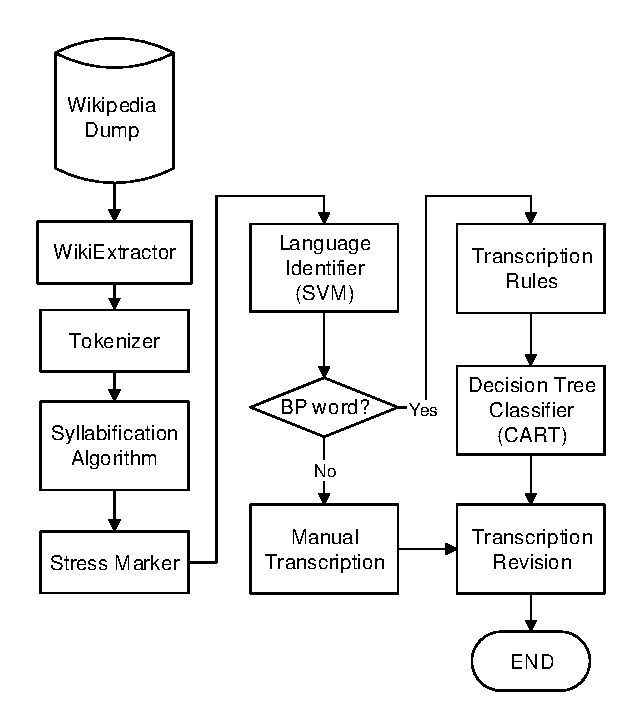
\includegraphics[width=8cm]{./gfx/aeiouado-flowchart-mod.pdf}}
\caption{{\it System architecture for building the pronunciation dictionary.}}
\label{g2p-architecture}
\end{figure}



\section{Method}

\subsection{Primary Word List}

We used the Portuguese Wikipedia's dump of 23\textsuperscript{rd} January 2014 as the primary word
list for the pronunciation dictionary. In order to obtain plain text from the articles, we employed WikiExtractor \cite{Wikiextractor2013};
it strips all the  MediaWiki markups and metadata forms. Afterwards, texts were tokenized and unique words types extracted. 
The Portuguese Wikipedia has about 168,8 million word tokens and 9,7 million types, distributed among  820,000 articles.
With the purpose of avoiding misspellings, URLs and other spurious data, only words with frequency higher than 10, 
which showed neither digits nor punctuation marks were selected. 

\subsection{Language Identifier}


A Language Identifier module was developed in order to detect loanwords in the pronunciation dictionary.
The Identifier consists of a Linear Support Vector Machine Classifier \cite{Steinwart2008} and was implemented in Python, 
through Scikit-learn \cite{Scikit2011}. It was trained on a corpus made of the 200,000, containing 100,000 Brazilian Portuguese
words and 20,000 words of each of the following languages: English, French, German, Italian and Spanish. All of these words were 
collected through web crawling News' sites and were not revised.
We selected these languages because they are the major donors of loanwords to Brazilian
Portuguese \cite{Alves2001}. From these words we extracted features such as initial and final bi- and trigraphs; 
number of accented graphs, vowel-consonant ratio; average mono-, bi- and trigraphs probability; and used 
them to estimate the classifier. Further details can be found in the website of the Project\footnote{http://nilc.icmc.usp.br/listener/aeiouado}. After training,
we applied the classifier to the Wikipedia word list with the purpose of identifying
loanwords among data. The identified loanwords were then separated from the rest of words for later 
revision, i.e. they were not submitted to automatic transcription.

\subsection{Syllabification algorithm and stress marker}

Our syllabification algorithm follows a rule-approach and is based straightforwardly on the syllabification
rules described in the Portuguese Language Orthographic Agreement \cite{Acordo2009}. Given space limitations,
rules were omitted from this paper as they can be found in the website of the project, along with all the
resources developed for the dictionary. As for the stress marker, once the syllable structure is known
in Brazilian Portuguese, one can predict where stress falls. Stress falls:

\begin{enumerate}
 \item on the antepenultimate syllable if it has an accented vowel $<$\'a,\^a,\'e,\^e,\'i,\'o,\^o,\'u$>$;
 \item on the ultimate syllable if it contains the accented vowels $<$\'a,\'e,\'o$>$ or $<$i,u$>$; or if it ends with one of the following consonants $<$r,x,n,l,z$>$;
 \item on the penultimate syllable otherwise.
\end{enumerate}


\subsection{Transcriber}
The transcriber is based on a hybrid approach, making use of manual transcription rules and an automatic classifier, 
which builds Decision Trees. Initially, transcription rules are applied to the words. 
The rules covers not all possible graphemes
to phoneme relations, but only those which are predictable by context. The output of the rules is what we called the 
intermediary transcription form. After obtaining it, a machine learning classifier is applied in order to
predict the transcription of the remaining graphemes. Figure 2 gives an example of the transcription process.

\begin{figure}[!ht]
\centerline{ 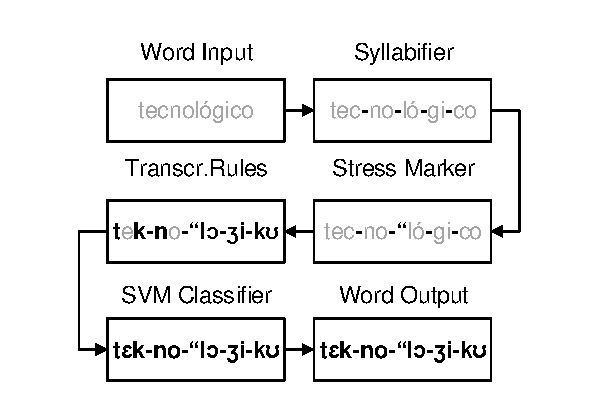
\includegraphics[width=8cm]{./gfx/aeiouado-transcript-ex.pdf}}
\caption{{\it Example of the transcription procedure -- in grey: graphemes yet to be transcribed; in black: graphemes already transcribed.}}
\label{transcExample}
\end{figure}

The rules' phase has two main goals: guarantee the correct transcription of certain predictable graphemes (mostly consonants)
and also ensure the alignment between graphemes and phones for the classifier. They were set in order to avoid
overlapping and order conflicts. Long sequences of graphemes, such as triphthongs, contextual diphthongs and general 
diphthongs are transcribed first (e.g.  $<$x-ce$> \rightarrow $\textipa{[-se]}). 
Then graphemes involving phones that undergo phonological processes are transcribed (e.g. $<$ti$> \rightarrow $\textipa{[tSi]},
$<$di$> \rightarrow $\textipa{[dZi]}). After that, several contextual and general monophones are transcribed 
(e.g. $<$\#x$> \rightarrow $\textipa{[S]}, $<$\#e-x$> \rightarrow $\textipa{[}\#\textipa{e-z]}). 

On what regards to the classifier, it was developed primarily to deal with the transcription of vowels. In Brazilian
Portuguese, vowels have a very irregular behavior, specially the mid ones. Therefore the relations between the vowels' 
graphemes and their corresponding phonemes are hard to predict beforehand through rules. Consider, for instance, the words 
``teto'' \emph{(roof)} and ``gueto'' \emph{(ghetto)}; both are nouns and share basically the same orthographic environment.
However the former is pronounced with an open ``e'' \textipa{["tE.tU]} and the latter with a closed one \textipa{["ge.tU]}.
The classifier employs Decision Trees, through an optimised version of the CART (Classification and Regression Trees)
algorithm and was implemented in Python, by means of the Scikit-learn library \cite{Scikit2011}. 

The algorithm was trained over a corpus of 3,500 words phonetically transcribed and manually revised, with a total
of 39,934 instances of phones. The feature extraction happened in the following way. After reviewing the data, we obtained the intermediary 
transcription form for each of these words and aligned them with the manual transcription. Then, we split
the intermediary transcription form into its corresponding phones and, for each phone, we extracted the following 
information: i) the phone itself; ii) 8 previous phones; iii) 8 following phones; iv) the distance between 
the phone and the tonic syllable; v) word class -- parts of speech; v) the manually transcribed phone. We considered
a window of 8 phones in order deal with vowel harmony phenomena. By establishing a window with such length, one 
can assure that pretonic phones will be able to reach the transcription of the vowels in the stressed syllable.
The classifier was applied to all 108,389 words categorized as BP words by the Language Identifier module,
all of them were cross-checked by two linguists with experience in Phonetics and Phonology.

\section{Results}

The Portuguese Wikipedia has about 168,8 million word tokens and 9,7 million types, distributed among 820k articles.
After applying the filters to the data, i.e. words with frequency higher than 10, with no digits nor punctuation marks,
we ended up with circa 238k word types, representing 151,9 million tokens. Table 1 describes the data.

\begin{table} [t,h]
\caption{\label{wikipedia} {\it Portuguese Wikipedia Summary -- Dumped on 23\textsuperscript{rd} January 2014.}}
\vspace{2mm}
\centerline{
\begin{tabular}{|ccc|}
\hline \bf & \bf Word Tokens  & \bf Word Types\\\hline
Wikipedia & 168,823,100 & 9,688,039 \\
Selected  & 151,911,350 & 238,012 \\
\textbf{\% Used} &90.0 & 2.4 \\
\hline
\end{tabular}}
\end{table}

The selected words covers 90,0\% of the Wikipedia content. Although the number of selected word types seems too small at first glance,
one of the reasons is that 
7,901,277 of the discarded words were numbers (81,5\%). The remaining discarded words contained misspellings (\emph{dirijem-se} --
it should be \emph{dirigem-se}), used a non-Roman alphabet ($\lambda$\emph{\'o}$\gamma \omega$), were proper names (\emph{Stolichno}, \emph{Z\'e-pereira}), 
scientific names (\emph{Aegyptophitecus}), abbreviations or acronyms (LCD, HDMI). 

As for the language identifier, we trained and evaluated it with the 200,000 words multilingual corpus. The corpus consists of
100,000 Brazilian Portuguese words and 20,000 words from each of the following languages: English, French, German, Italian and Spanish. 
All of these words were collected through web crawling News' sites and were not revised.
The results obtained for the identifier, through 5-fold cross validation are described in Table 2. 

\begin{table} [t,h]
\caption{\label{langIdentEval} {\it Results from the Language Identifier module -- Training Phase.}}
\vspace{2mm}
\centerline{
\begin{tabular}{|ccccc|}
\hline
 & \textbf{Precision} & \textbf{Recall} & \textbf{F1-score} & \textbf{Support} \\ \hline
BP words & 0.85 & 0.89 & 0.87 & 100,000 \\ 
Foreign Words & 0.88 & 0.84 & 0.86 & 100,000 \\
\bf Avg/Total & 0.86 & 0.86 & 0.86 & 200,000 \\ \hline
\end{tabular}}
\end{table}

The classifier showed an average F1-score of 0.86. Although such result is not as good as we expected -- some authors
reported 99\% by using similar methods with trigrams probability, the relatively low F1-score can be explained given
the nature of the data. In most language identifiers, the input  consists of texts or several sentences, in other 
words, there is much more data available for the classifier. Since we are working with single words, the confusion
of the model is higher and the results are, consequently, worse. Additionally, because the word list used to train the identifier
was not revised, there is noise among the data. After training and evaluating the classifier,
we applied it to the selected word list derived from the Wikipedia, in order to detect loanwords. Table 3 
describes the results gathered.

\begin{table} [t,h]
\caption{\label{langIdentWiki} {\it Results from the Language Identifier module -- Wikipedia word list.}}
\vspace{2mm}
\centerline{
\begin{tabular}{|cc|}
\hline
 & \textbf{Wikipedia word list}\\ \hline
BP words & 108,370 (46\%)\\ 
Foreign Words & 129,642 (54\%)\\
\bf Total & 238,012 \\ \hline
\end{tabular}}
\end{table}

As one can observe, although we established a frequency filter to avoid spurious words, many loanwords
still remain. More than half of the word list selected from Wikipedia consists of foreign words. Notwithstanding 
that, the list of Brazilian Portuguese words is still of considerable size. For instance, the CMUdict \cite{CMUdict1998}, a reference
pronunciation dictionary for the English language, has about 125,000 word types.

Concerning the syllabification algorithm and the stress marker, we did not evaluate them in isolation, but together with 
the transcriber since the rules for each of these modules are intertwined.
That is to say the transcription rules are strictly dependent on the stress marker module and the syllable identifier. Besides,
the Decision Tree Classifier is built upon the output of the transcription rules, so it is entirely dependent on it.
The Decision Tree Classifier was trained over a corpus of 3,500 cross-checked transcribed words, containing 39,934 instances of phones.
We analyzed its performance through 5-fold cross validation, the results for each individual phone are summarized in Table 4.

\begin{table} [t,!h]
\caption{\label{transcriberEval} {\it Results from the Transcriber -- Training Phase.}}
\vspace{2mm}
\centerline{
\begin{tabular}{|ccccc|}
\hline
 & \bf Precision & \bf Recall & \bf F1-score & \bf Support \\ \hline
\emph{syl. boundary} & 1.00 & 1.00 & 1.00 & 9099 \\ 
\emph{stress} & 1.00 & 1.00 & 1.00 & 3507 \\ 
\textipa{p} & 1.00 & 1.00 & 1.00 & 760 \\ 
\textipa{b} & 1.00 & 1.00 & 1.00 & 357 \\ 
\textipa{t} & 0.99 & 0.99 & 0.99 & 1135 \\ 
\textipa{d} & 0.99 & 0.99 & 0.99 & 1148 \\ 
\textipa{k} & 0.99 & 0.99 & 0.99 & 978 \\ 
\textipa{g} & 1.00 & 1.00 & 1.00 & 298 \\ 
\textipa{tS} & 0.98 & 0.98 & 0.97 & 450 \\ 
\textipa{dZ} & 0.96 & 0.96 & 0.96 & 243 \\ 
\textipa{m} & 1.00 & 1.00 & 1.00 & 668 \\ 
\textipa{n} & 1.00 & 1.00 & 1.00 & 556 \\ 
\textipa{\textltailn} & 1.00 & 1.00 & 1.00 & 69 \\ 
\textipa{f} & 1.00 & 1.00 & 1.00 & 311 \\ 
\textipa{v} & 1.00 & 1.00 & 1.00 & 531 \\ 
\textipa{s} & 0.98 & 0.98 & 0.98 & 2309 \\ 
\textipa{z} & 0.93 & 0.94 & 0.93 & 416 \\ 
\textipa{S} & 0.84 & 0.84 & 0.84 & 138 \\ 
\textipa{k.s} & 0.72 & 0.64 & 0.66 & 41 \\ 
\textipa{Z} & 1.00 & 1.00 & 1.00 & 196 \\ 
\textipa{l} & 1.00 & 1.00 & 1.00 & 682 \\ 
\textipa{L} & 1.00 & 1.00 & 1.00 & 58 \\ 
\textipa{R} & 1.00 & 1.00 & 1.00 & 1388 \\ 
\textipa{h} & 0.98 & 0.99 & 0.99 & 737 \\ 
\textipa{H} & 0.97 & 0.92 & 0.94 & 169 \\ 
\textipa{w} & 0.97 & 0.98 & 0.97 & 441 \\ 
\textipa{\~w} & 0.98 & 0.99 & 0.99 & 309 \\ 
\textipa{j} & 0.97 & 0.95 & 0.96 & 223 \\ 
\textipa{\~j} & 0.95 & 1.00 & 0.98 & 110 \\ 
\textipa{a} & 1.00 & 1.00 & 0.99 & 2316 \\ 
\textipa{@} & 0.99 & 0.99 & 0.99 & 1093 \\ 
\textipa{E} & 0.65 & 0.68 & 0.66 & 275 \\ 
\textipa{e} & 0.93 & 0.91 & 0.92 & 1779 \\ 
\textipa{i} & 0.98 & 0.99 & 0.98 & 2073 \\ 
\textipa{I} & 0.97 & 0.97 & 0.97 & 365 \\ 
\textipa{O} & 0.69 & 0.75 & 0.71 & 220 \\ 
\textipa{o} & 0.93 & 0.92 & 0.93 & 1112 \\ 
\textipa{u} & 0.96 & 0.96 & 0.96 & 488 \\ 
\textipa{U} & 1.00 & 1.00 & 1.00 & 1033 \\ 
\textipa{\~a} & 1.00 & 1.00 & 1.00 & 719 \\ 
\textipa{\~e} & 0.96 & 0.97 & 0.97 & 497 \\ 
\textipa{\~i} & 0.99 & 0.99 & 0.99 & 274 \\ 
\textipa{\~o} & 0.97 & 0.96 & 0.97 & 299 \\ 
\textipa{\~u} & 0.94 & 0.92 & 0.93 & 64 \\ 
Avg/Total & 0.98 & 0.98 & 0.98 & 39934 \\ \hline
\end{tabular}}
\end{table}

As it can be seen, the method achieved very good results, with a F1-score of 0.98. Many segments were transcribed
with 100\% accuracy, most of them were consonants. As it was expected, the worst results are related to mid vowels 
\textipa{[E, e, O, o]}, specially mid-low vowels, \textipa{[E]} showed a F1-score 0.66 and \textipa{[O]} of 0.71. It 
can be the case that since the grapheme context is the same for \textipa{[E, e]} and \textipa{[O, o]}, the Decision
Tree classifier generalizes, in some cases, to the most frequent phone, that is the mid-high vowels \textipa{[e,o]}.
The transcriber also had problems with the \textipa{[k.s]} (F1-score: 0.66) and \textipa{[S]} (F1-score: 0.84). This 
result was also expected, both these phones are related to the grapheme $<$x$>$ which, in Brazilian Portuguese,
shows a very irregular behavior. In fact, $<$x$>$ can be pronounced as \textipa{[S, s, z, k.s]}, depending on the 
word:  ``bruxa'' \emph{(witch)} \textipa{[S]}, ``pr\'oximo'' \emph{(near)} \textipa{[s]};  ``exame'' \emph{(test)}
\textipa{[z]} and ``axila'' \emph{(armpit)} \textipa{[k.s]}.

\section{Final Remarks}

We presented the method we employed in building a pronunciation dictionary for Brazilian Portuguese. High F1-score 
values were achieved while transcribing most of the graphemes in Brazilian Portuguese and the dictionary can be
considered robust enough for Large Vocabulary Continuous Speech Recognition (LVCSR) and Speech Synthesis. Although 
the rules we developed are language-specific, the architecture we used for compiling the dictionary, by using transcription
rules and machine learning classifiers, can be successfully replicated in other languages. In addition, the entire dictionary,
all scripts, algorithms and corpora were made publicly available.

\section{Acknowledgements}
Part of the results presented in this paper were obtained through research activity in the project titled 
``Semantic Processing of Brazilian Portuguese Texts'', sponsored by \emph{Samsung Eletr\^onica da Amaz\^onia Ltda.} under 
the terms of Brazilian federal law number 8.248/91.




\paragraph{Further developments}

Since the publishing date of our paper (\citeauthor{Mendonca2014}~\cite{Mendonca2014}), Aeiouad\^o \ac{G2P} has been improved. Recently, we increased the training database to XXX words (XXX phone tokens). Moreover we are now using extra morphological information in order to determine the grapheme's transcription, mostly to solve the problems with the mid vowels \textipa{[E, e, O, o]}. 

Previously we were using only the parts of speech as the source of morphological information. We assumed that by just providing the words' parts of speech, the Decision Tree Classifier would be able to learn and differ pairs of heterophonic homographs, such as ``jogo'' \textsc{noun} \emph{(game)} and ``jogo'' \textsc{verb} \emph{(I play)}, or ``governo'' \textsc{noun} \emph{(government)} and ``governo'' \textsc{verb} \emph{(I rule)}. However, given the poor performance of the conversor in discerning between \textipa{[E]} vs. \textipa{[e]}, and \textipa{[O]} vs. \textipa{[o]}; we decided to refine the morphological features. 

We adapted the training database to the Unitex-PB dictionary \cite{Muniz2004}, which follows  formalismo DELA (Dictionnarie Electronique du LADL)

There is a huge lexicon with,

This type of alternation is very productive in \ac{BP}.  reported to have collected 1,812 pairs of heterophonic homographs in dictionaries and , although only 226 occurred in corpus).

\citeauthor{}, Pandu , although in a corpus analysis, only 226 \cite{Shulby2013}.

However this is not the case. Previously, only the word class information was used to determine. We thought that would be enough to 


%*****************************************
%*****************************************
%*****************************************
%*****************************************
%*****************************************